% !TeX root = ../main.tex
\documentclass[./../main.tex]{subfiles}

\begin{document}

Ứng dụng được phát triển từ nhu cầu thực tế của thành viên trong nhóm, các cá nhân thích đọc truyện tranh. Trong đó, việc đọc truyện với UI/UX tốt, chất lượng tốt là mục tiêu của nhóm trong việc phát triển. Với vai trò và mục tiêu trên, nhóm đã phân tích vấn đề thành các đơn vị nhỏ hơn sau.

\subsection{Đối tượng sử dụng}

Hệ thống có 3 đối tượng sử dụng chính.

\begin{description}
	\item[Khách vãng lai đọc truyện] Bất kỳ người dùng truy cập website, ứng dụng di động có thể đọc các truyện trên hệ thống. Mục đích đối với nhóm người này là có thể nhanh chóng đọc truyện được thông qua việc chia sẻ của bạn bè thông qua mạng xã hội, đường dẫn liên kết hay chỉ với tên của Website.
	\item[Người dùng đọc truyện] Người dùng của hệ thống cho phép đọc truyện, theo dõi, nhận thông báo,...và các tính năng khác của hệ thống. Nhóm người này có mục đích thường xuyên đọc và theo dõi truyện từ  hệ thống muốn nhận được thêm các thông báo khi có nội dung mới được đưa ra. Đi kèm với đó là sử dụng các tính năng khác mang tính cá nhân như là theo dõi được lịch sử đọc truyện, lưu lại truyện hay đọc,…
	\item[Quản trị viên] Người quản trị nội dung hệ thống, người dùng. Đồng thời cũng là người tạo ra các truyện dựa trên sự ủy quyền của tác giả. Nhóm người này có mục đích chính là quản trị hệ thống cả về nội dung và con người để đảm bảo hệ thống diễn ra đảm bảo nhất. Các nội dung được đăng trên hệ thống cần thông qua nhóm người dùng này.
\end{description}

\subsection{Yêu cầu chức năng}

Dựa vào các nhóm người dùng trên, các yêu cầu chức năng được đặt ra là
\begin{itemize}
	\item Cho phép xem, đọc nội dung của của truyện tranh.
	\item Tìm hiểu thông tin về tác giả.
	\item Cho tìm kiếm truyện.
	\item Bình luận về truyện.
	\item Nhận thông báo về truyện.
	\item Lưu lại các bộ truyện yêu thích.
	\item Đăng nhập, đăng ký
	\item Hiển thị các trang truyện theo đúng thứ tự
	\item Người dùng có thể chuyển chap, chỉnh chế độ đọc, ...
	\item Lưu trữ danh sách yêu thích
	\item Đăng truyện mới
	\item Đăng chap truyện mới
	\item Dark mode
	\item Báo cáo lỗi truyện
	\item Đa ngôn ngữ (i18next)
	\item Nhận thông báo chap mới
\end{itemize}

\subsection{Yêu cầu phi chức năng}

Dựa vào nhu cầu của người dùng, nhóm định nghĩa được 4 yêu cầu phi chức năng cho sản phẩm.

\subsubsection{Tính khả dụng}

Đáp ứng > 90\% trên toàn bộ mẫu người sử dụng dùng có thể...
\begin{itemize}
	\item Có thể sử dụng hệ thống trong 5 phút.
	\item Đăng ký trong vòng 5 phút.
	\item Đăng nhập trong vòng 1 phút.
	\item Tìm kiếm truyện và đọc được truyện trong vòng 1 phút.
\end{itemize}

\subsubsection{Tính sẵn sàng}

Đáp ứng thời gian vận hành liên tục trên 98\%.

\subsubsection{Hiệu suất}

\begin{itemize}
	\item Đáp ứng ít nhất cho 5.000 CCU.
	\item Đáp ứng 95\% số yêu cầu dưới 5s.
	\item Trung bình thời gian phản hồi mỗi yêu cầu là dưới 2s.
\end{itemize}

\subsubsection{Bảo mật}

Khả năng bảo vệ hệ thống trước tấn công DDoS, hạn chế các lỗ hổng nguy hiểm. Đảm bảo bảo mật về thông tin cá nhân.

\subsection{Mô hình ca sử dụng}

Dựa vào các yêu cầu đối với các nhóm đối tượng ở trên, nhóm đã mô hình hóa thành các Tác nhân đối với hệ thống.

Ngoài ra, Firebase được triển khai như một hệ thống ngoài của hệ thống nên sẽ được coi là một tác nhân cần tương tác với hệ thống.

\begin{figure}[H]
	\centering
	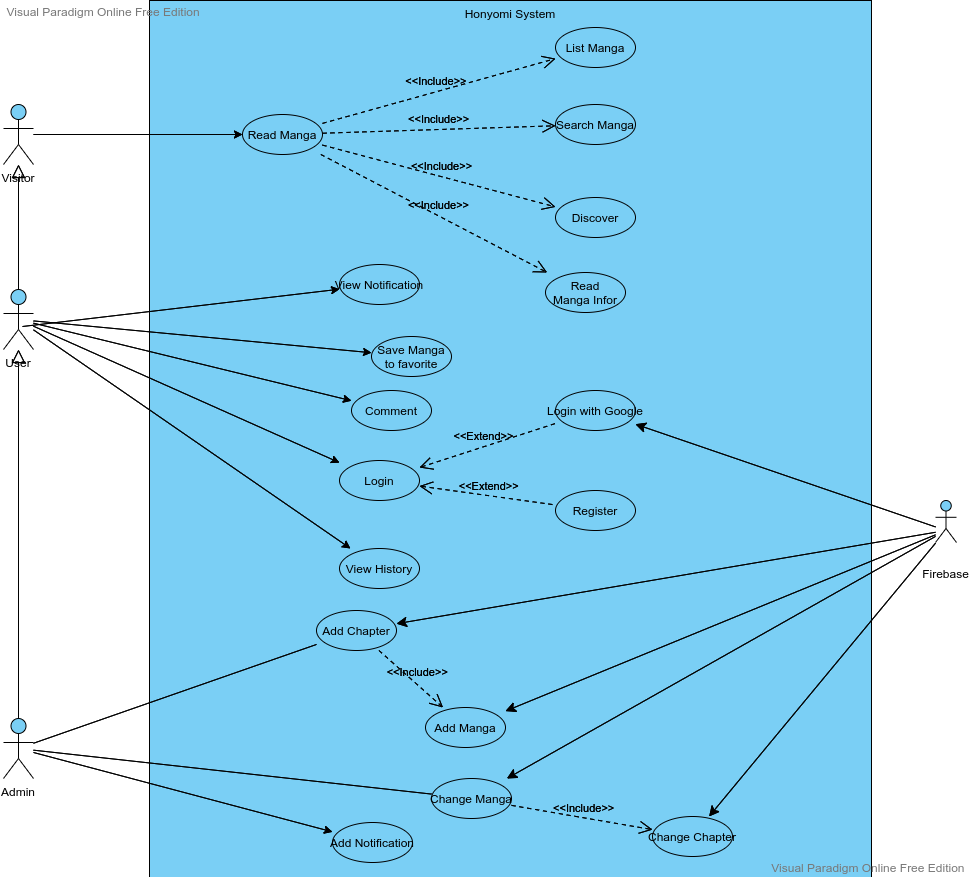
\includegraphics[width=\linewidth]{./images/image6.png}
	\caption{Biểu đồ ca sử dụng}
\end{figure}

\subsubsection{Đăng nhập và đăng ký}
Người dùng có thể đăng nhập tài khoản thông qua 2 cách:
\begin{itemize}
\item Bằng email/username và mật khẩu.
\item Bằng tài khoản Google.
\end{itemize}
Người dùng vẫn có thể sử dụng hệ thống mà không cần đăng nhập.
Tuy nhiên, họ sẽ không thể truy cập được vào các tính năng mang tính cá nhân
\begin{itemize}
\item Lưu trữ danh sách truyện yêu thích
\item Gửi bình luận cho chap truyện.
\item Đọc truyện
\end{itemize}
Người dùng có thể chọn một quyển truyện bất kỳ trên hệ thống.
Sau đó, họ sẽ chọn chương mình muốn đọc và hệ thống sẽ hiển thị danh sách các trang cho người dùng.
Các chương được hiển thị sẽ phụ thuộc vào cài đặt và locale của người dùng. (V.D. Hệ thống hiển thị chương truyện có ngôn ngữ tiếng Việt cho một người dùng ở Việt Nam). 


Yêu cầu
\begin{itemize}
\item Về việc hiển thị chương
\item Người dùng có thể chọn thủ công ngôn ngữ của các chương
\end{itemize}
Hệ thống cần hiển thị chương với ngôn ngữ tiếng Anh nếu chương với ngôn ngữ người dùng không tồn tại.
\subsubsection{Về việc hiển thị trang truyện}
\begin{itemize}
\item Hệ thống cần cung cấp khả năng customize tối thiểu 2 yếu tố sau:
\item Thứ tự trang (trái sang phải, phải sang trái, trên xuống dưới).
\item Page Fit (Fit theo chiều ngang và chiều dọc)
\item Giao diện trang đọc truyện cần tối giản.
\item Trang truyện phải được hiển thị bằng skeleton trước khi load ảnh, để tránh vỡ layout.
\item Tìm kiếm (và filter) truyện
\end{itemize}


Người dùng có thể tìm kiếm truyện trên hệ thống theo tên và filter theo các tiêu chí:
\begin{itemize}
\item Tác giả
\item Thể loại
\item Trạng thái
\item Danh sách truyện có thể được sắp xếp theo:
\item Tên truyện
\item Thời gian ra mắt
\item Lướt xem
\end{itemize}
Yêu cầu: Danh sách truyện cần được phân trang trước khi trả về cho người dùng.
\subsubsection{Lưu truyện vào danh sách yêu thích}
Người dùng cá nhân có thể lưu truyện trên hệ thống vào danh sách yêu thích của mình.

Người dùng có thể xem danh sách này bất cứ lúc nào.


Tác nhân: Người dùng cá nhân (user)
\subsubsection{Xem truyện trong danh sách yêu thích}
Người dùng cá nhân có thể xem và tìm kiếm truyện theo tên trong danh sách yêu thích.

Tác nhân: Người dùng cá nhân (user)
\subsubsection{Xem lịch sử đọc truyện}
Tác nhân: Người dùng cá nhân
\begin{itemize}
\item Người dùng cá nhân có thể xem lịch sử đọc truyện của mình. Với mỗi truyện, hệ thống sẽ lưu trữ các thông tin sau:
\item Thời gian đọc truyện gần đây nhất
\item Chương truyện đã đọc gần đây nhất
\end{itemize}
Với mỗi chương truyện, hệ thống sẽ lưu các thông tin sau: Đã đọc chương truyện này hay chưa.
\subsubsection{Báo cáo lỗi truyện}
Hệ thống sẽ tự động gửi báo cáo về BE khi một trang truyện không load được. Thông tin gửi bao gồm:


Tác nhân: không có
\begin{itemize}
\item IP người dùng?
\item Đường dẫn đến trang truyện bị lỗi.
\item Đường dẫn dùng để load trang truyện bị lỗi.
\end{itemize}
Thông tin này sẽ được lưu lại và hiển thị cho quản trị viên để có phương án phù hợp.
\begin{itemize}
\item Cài đặt cá nhân
\item Người dùng có thể cài đặt các thông tin sau: Email, Mật khẩu và Các cài đặt cá nhân.
\end{itemize}
\subsubsection{Tạo truyện mới}
Quản trị viên có thể tạo truyện mới bằng giao diện admin của hệ thống.
QTV sẽ nhập vào thông tin cơ bản, hệ thống sẽ thực hiện validate các thông tin đó và gửi lên backend server.
Sau đó, hệ thống sẽ hiển thị tin nhắn thành công hoặc thất bại.


Tác nhân: Quản trị viên


Thông tin để tạo truyện bao gồm:
\begin{itemize}
\item Tên truyện (có thể thêm nhiều tên cho từng ngôn ngữ)
\item Tên phiên âm (romaji) của truyện
\item Tên quốc tế (tiếng Anh) của truyện
\item Độ tuổi
\item Mô tả?
\item Danh sách tác giả
\item Danh sách thể loại
\item Loại manga (manhwa, manga, manhua, doujin, …)
\item Trạng thái (ongoing, finished, dropped)
\end{itemize}
Yêu cầu
\begin{itemize}
\item Cần cung cấp tên truyện cho ít nhất 1 ngôn ngữ
\item Cần có checkbox để đánh dấu truyện thuộc thể loại nsfw.
\end{itemize}
\subsubsection{Thêm chương truyện}
Quản trị viên có thể thêm chương truyện cho một truyện có sẵn.

Tác nhân: Quản trị viên


Thông tin chương truyện bao gồm:
\begin{itemize}
\item Tên chương truyện (nhiều ngôn ngữ)
\item Danh sách link các trang truyện
\item Ngôn ngữ của chương truyện (sau khi dịch)
\item Số của chương truyện
\item url đến thumbnail của chương?
\end{itemize}
\subsubsection{Sửa chương truyện}
\begin{itemize}
\item Quản trị viên có thể sửa thông tin của chương truyện. Thông tin có thể sửa:
\item Tên chương truyện (nhiều ngôn ngữ)
\item Danh sách link các trang truyện
\item Ngôn ngữ của chương truyện (sau khi dịch)
\item Số của chương truyện
\item url đến thumbnail của chương?
\end{itemize}

Tác nhân: Quản trị viên
\subsubsection{Gửi thông báo}
Quản trị viên có thể gửi thông báo đến người thông qua Email về thông tin Chapter mới, Manga mới được ra mắt.


Tác nhân: Quản trị viên
\subsubsection{Xem danh sách báo cáo lỗi}
Quản trị viên có thể xem danh sách báo cáo lỗi load truyện và resolve nó sau khi đã giải quyết xong vấn đề.


Tác nhân: Quản trị viên


Yêu cầu
\begin{itemize}
\item Quản trị viên có thể hoàn tác sau khi bấm resolve để tránh bấm nhầm.
\item Không xóa báo cáo cũ.
\item Cho phép resolve hàng loạt.
\end{itemize}


\end{document}